 \documentclass[final,5p,times,twocolumn,authoryear]{elsarticle}

\usepackage{amssymb}
\usepackage{mathabx}
\usepackage{physics}
\usepackage{multicol}

\journal{CTA200}

\begin{document}

\begin{frontmatter}

\title{Tidal evolution of the Earth - Moon system}

\author[first]{Daniel Rogojanski}
\affiliation[first]{{University of Toronto}}

\begin{abstract}
This paper presents the results of the final project done in the CTA200 course. Graphical representations will be presented with a simple model of the Earth-Moon system, including the history of angular momentum, spin, day length and lunar semi-major axis.
\end{abstract}

\end{frontmatter}

\section{Set-up}

The setup for this paper included coding all of the variables, i.e. gravitational constant. These values were then run through a unit converter to homogenize the units (into SI units) and then create a second set of variables expressed with units of years as opposed to seconds. Throughout this project, the SI unit system (with the addition of the unit years) was implemented. The addition of the unit years was used to simplify the integration over billions of years. For all mentions of variables, a list has been made at the end of this paper which contains all variables, units and values used throughout. 

\section{Present values and timescales}

Using the given formulas, the initial values of the Earth's angular momentum, spin and lunar angular momentum were calculated. These values were then used to calculate Lunar and solar tidal torques. All of these values are given in Table 1.

\begin{table}[htb]
\centering
\begin{tabular}{l c c} 
 \hline
 Variable & Value & Units \\ 
 \hline
 Earth\,Orbital\,Angular\,Momentum & $2.6e40$ & $(kg\ m^2)/s$ \\ 
 Earth\,Angular\,Spin & $5.8e33$ & $(kg\ m^2)/s$ \\ 
 Lunar\,Orbital\,Angular\,Momentum & $2.9e34$ & $(kg\ m^2)/s$ \\
 Lunar\,Torque & $4.6e16$ & Nm \\
 Solar\,Torque & $9.8e15$ & Nm \\
 \hline
\end{tabular}
\caption{These values were calculated by using the formulas provided in the CTA200 final assignment page. For simplicity, the equations have been omitted from this paper.
}
\label{Table1}
\end{table}

Using these values, timescale estimates were calculated for the time it takes for a variable to double in magnitude. All values are presented in Table 2. As seen in the timescales, the time to double the Earth's angular spin is of the lowest magnitude, which makes sense as changing the angular spin of the Earth must take less energy than changing its orbital angular momentum. Earth's orbital angular momentum is expected to be the largest as the Earth has a very large inertia and the solar torque is not strong enough to have a short-term effect on the Earth's orbit. It is important to note that since the timescales for Earth's spin and the lunar angular momentum are similar, their graphs should have similar general timescale properties. 

\begin{table}[htb]
\centering
\begin{tabular}{l c c} 
 \hline
 Property & Timescale & Unit \\ 
 \hline
 Earth\,Orbital\,Angular\,Momentum & $8.6e16$ & Years \\ 
 Earth\,Angular\,Spin & $3.3e9$ & Years \\ 
 Lunar\,Orbital\,Angular\,Momentum & $2.0e10$ & Years \\
 \hline
\end{tabular}
\caption{This table shows the estimated timescales for various properties to double in magnitude.
}
\label{Table2}
\end{table}

\section{Earth-Moon relationship throughout time}

Using a differential equation solver solve\_ivp, the three parameters $\dv{L_\Earth}{t}$, $\dv{S_\Earth}{t}$, $\dv{L_\leftmoon}{t}$ were integrated back in time until the magnitude of the values diverged. The result was plotted to graphically show the evolution of the properties throughout time. The resulting graphs are shown in Figure 1. 

\begin{figure}[!h]
	\centering 
	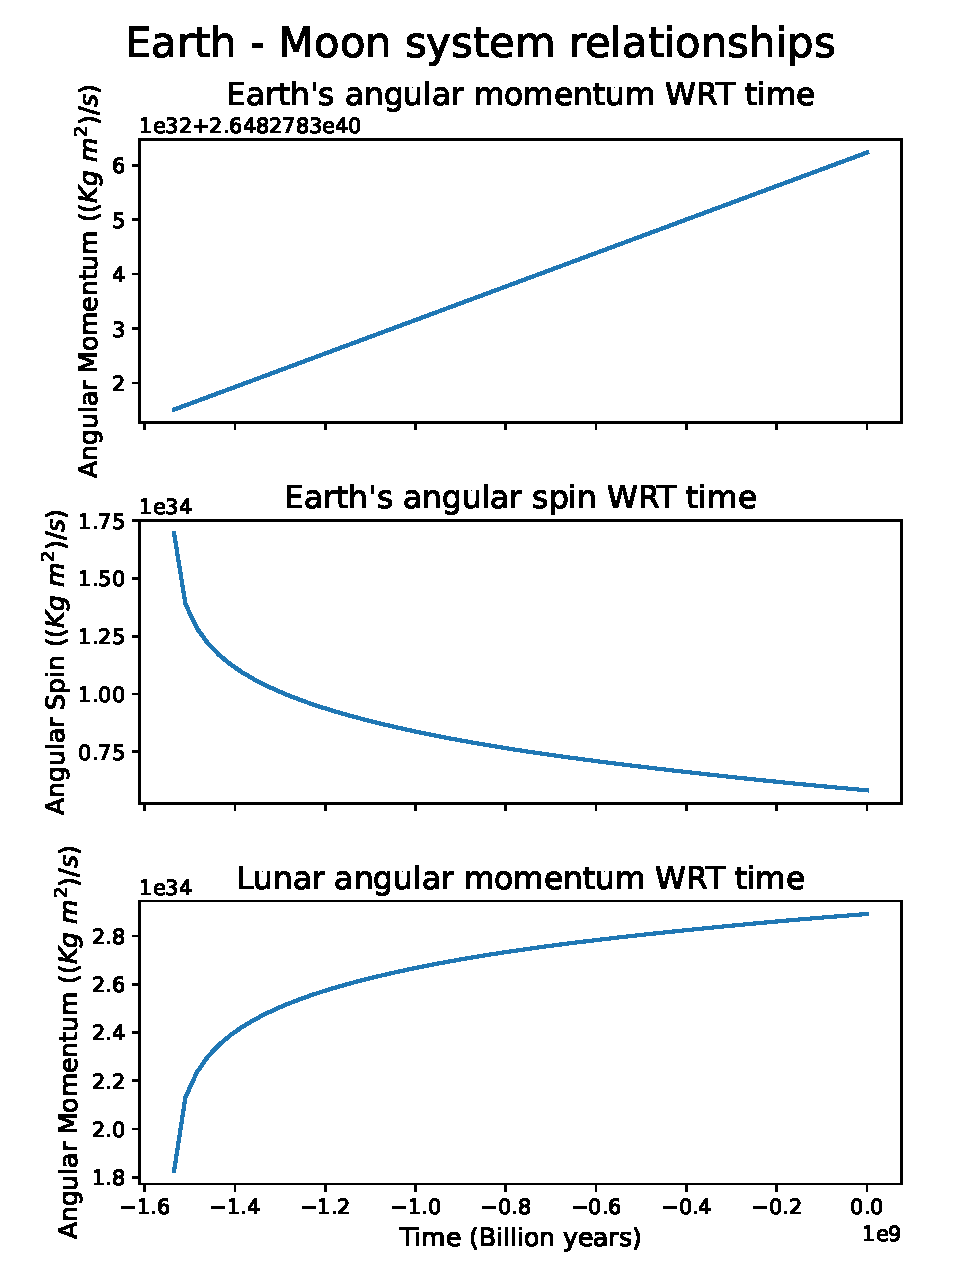
\includegraphics[width=0.4\textwidth]{Earth-Moon system relationships.pdf}	
	\caption{Evolution of the Earth-Moon system over billions of years} 
\end{figure}

According to the tidal model used, the moon would have formed approximately 1.5 billion years ago, which is not accurate as current estimates show that the moon (and Earth) would have formed around 4.5 billion years ago. This result matches an estimation done in the 1950s where a similar model was used. As seen, this model is lacking some strong parameter(s) that would lead to the actual age of the moon. Additionally, from this model, it can be noted that, throughout 1.5 billion years, the Earth's orbital angular momentum (top graph) was relatively unchanging, whereas the Earth's spin and lunar angular momentum had exponential and logarithmic changes, respectively. These properties drawn from the graphs correlate to the previously calculated timescales, where it was concluded that the Earth's spin and the lunar momentum would undergo noticeable changes over this period and the Earth's angular momentum would not.

\section{Lunar semi-Major axis}
From the basic model used, it is understood that the moon would have formed from a large body impact with the Earth, and since that point in time, the lunar semi-major axis would have been increasing. The current value of the lunar semi-major axis is 380000km, with a rate of change of 3 cm/year (Known values). By using the data from the Earth-Moon relationship, it was possible to graph the orbital distance of the moon as a function of time as shown in Figure 2.

\begin{figure}[!h]
	\centering 
	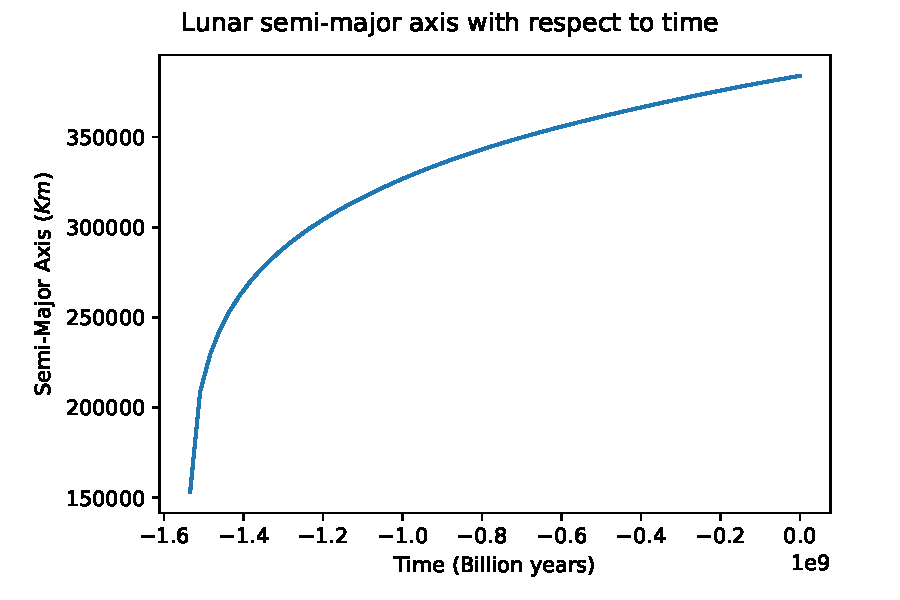
\includegraphics[width=0.48\textwidth]{semi major axis.pdf}	
	\caption{Lunar Semi-Major axis from its formation to present time} 
\end{figure}

This graph shows that the orbital axis is increasing, but its rate of change is decreasing. From this data, it was calculated that the current moon's semi-major axis increases by about 3.8 cm/year which is a close estimation. However, it should be noted that current estimates state that the moon would have formed around 18000 km from Earth, known as the Roche limit. This is not accurately represented in the graph as it caps out at 150,000 km, which is likely due to the same missing parameters mentioned earlier. 

\section{Earths history of day length}

Since it is known that the moon's orbit influences the Earth's angular velocity, it is expected that its velocity would have been much higher when the moon was closer to Earth. Using the lunar semi-major axis, it was possible to calculate the approximate day length in hours with respect to the Earth's age. The data is presented in Figure 3. 

\begin{figure}[!h]
	\centering 
	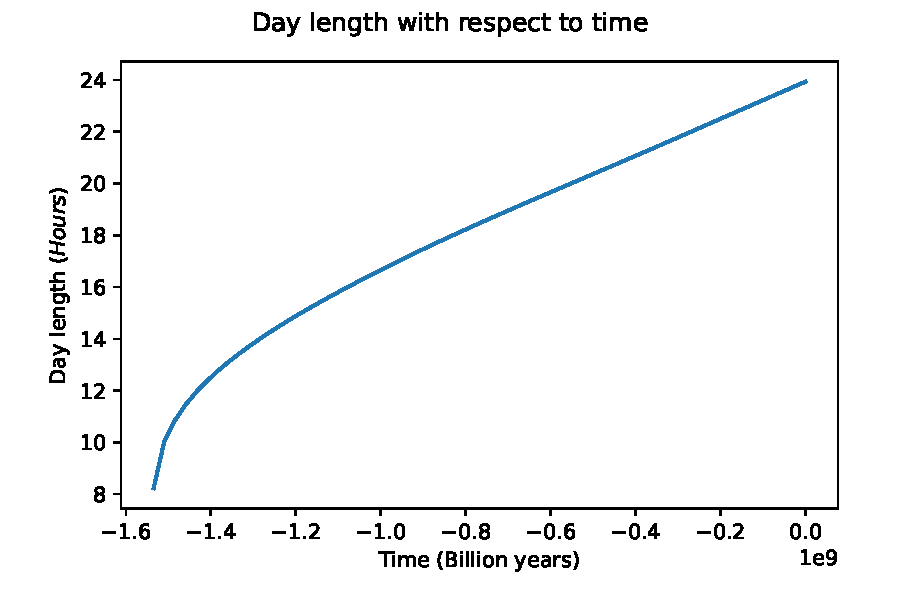
\includegraphics[width=0.48\textwidth]{Day length.pdf}	
	\caption{Earth's day lengths from its formation to present time} 
\end{figure}

From this data, it is expected that 1.5 billion years ago the day length would have been one-third of the present day length. However, since it is believed that the moon formed at the Roche limit, the day length at that value of separation was calculated to be 4.9 hours. This value is quite close to the generally accepted value of around 4 hours. 

\section{Improvements to the model}

As pointed out throughout this report, the estimation of the Earth-Moon system's age from this model is widely inaccurate. In this section, I will propose a few possible missed factors that could influence the model to generate a more generally accepted answer. Any of the following could be employed in the tidal/model equations and would likely lead to greater accuracy in the result.  

\subsection{Rigid body approximations and no internal forces}
In this model, it was approximated that the Earth and moon are rigid spherical bodies and that no atmospheric/ocean-related force plays into the model. However, it is known that the Earth is not spherical and has 2 ocean bulges due to the lunar torque on the Earth. Because of this, the ocean would likely apply some form of counter torque or friction onto the Earth, slowing it. Additionally, it is possible that atmospheric temperature would also play a role as temperature could affect the atmospheric density and therefore compound the aforementioned torque/friction forces.

\subsection{Idealisation of the systems properties}
For this model to be employed, it was assumed that the lunar orbit is equidistant from the Earth at all times. As expected, the exclusion of these properties simplifies the model, but, likely, having fluctuating torque values based on the distance to the moon as a function of time throughout the year, or perhaps an average distance would have some effect on the model's estimation. 

\subsection{External forces}
In this model, the only bodies considered were the sun, moon and Earth. While it is likely that other planetary bodies have little effect on the Earth-Moon system, it is possible that including gravitational forces from other planets in the solar system could lead to a slightly better calculation. The downside of including external forces is that the model would get a lot more complicated without leading to a huge change in the final result. 

\section{Conclusion}
From this simple model, it was concluded that the moon formed 1.5 billion years ago, at which point the moon would have been 150 thousand kilometres from the Earth, resulting in 8-hour days. This model has proven to be unreliable as current estimates put the formation of the moon at 4.5 billion years ago. This model correlates to the findings and conclusions from the first estimations of the moon's age in the 1950s, and it proves to have some missing factors. Overall, this assignment was very interesting and directly demonstrates that precision in the model is essential to yielding a good result. This assignment taught me a lot of computational astrophysics concepts and was a great introduction to the world of computational astrophysics research. 

\newpage
\section*{Appendix A. All variables used throughout the project}
\begin{table}[!h]
\centering
\begin{tabular}{l c c}
 \hline
 Variable & Value & Units \\ 
 \hline
 Earth\,Orbital\,Angular\,Momentum & $2.6e40$ & $(kg\,m^2)/s$ \\ 
 Earth\,Angular\,Spin & $5.8e33$ & $(kg\,m^2)/s$ \\ 
 Earth\,Angular\,Velocity & $7.3e-5$ & radians/s \\
 Earth\,Moment\,of\,Inertia & $8.0e37$ & $kg\,m^2$ \\
 Earth\,Love\,Number & 0.298 & N/A \\
 Earth\,Mass & $6.0e24$ & kg \\
 Earth\,Radius & $6.4e6$ & m \\
 Earth\,Semi-Major\,Axis & $1.5e11$ & m \\
 Lunar\,Orbital\,Angular\,Momentum & $2.9e34$ & $(kg\ m^2)/s$ \\
 Lunar\,Mass & $7.3e22$ & kg \\
 Lunar\,Semi-Major\,Axis & $3.8e8$ & m \\
 Lunar\,Torque & $4.6e16$ & Nm \\
 Lunar\,Current\,Recession\,Rate & 0.038 & m/year \\
 Solar\,Mass & $2.0e30$ & kg \\
 Solar\,Torque & $9.8e15$ & Nm \\
 Tidal\,Quality\,Factor & 11.5 & N/A \\
 Gravitation\,Constant & $6.67e-11$ & $(N\,m^2)/kg^2$ \\
 Day\,Length\,At\,Roche\,Limit & 4.9 & Hours \\
 \hline
 Variables represented in years & Value & Units \\ 
 \hline
 Earth\,Orbital\,Angular\,Momentum & $8.4e47$ & $(kg\,m^2)/year$ \\
 Earth\,Angular\,Spin & $1.8e41$ & $(kg\,m^2)/year$ \\ 
 Earth\,Angular\,Velocity & $2.3e3$ & radians/year \\
 Lunar\,Orbital\,Angular\,Momentum & $9.1e41$ & $(kg\,m^2)/year$ \\
 Lunar\,Torque & $4.6e31$ & $(kg\,m^2)/year^2$ \\
 Solar\,Torque & $9.7e30$ & $(kg\,m^2)/year^2$ \\
 Gravitation\,Constant & $6.64e4$ & $m^3/(kg\,year^2)$ \\
 \hline
\end{tabular}
\caption{These values were used for all calculations throughout the production of this paper, some values are known constants like the gravitational constant, and some were calculated like the lunar torque.
}
\end{table}


\end{document}

